%%%*******************************************************************************
%  Classe Latex THEOPRAX, Version 0.0.0 31/10/2017
%
%  Define as normas e estilo das dissertações, teses ou tcc do SENAI CIMATEC
%
%%%-------------------------------------------------------------------------------

%%%-------------------------------------------------------------------------------
% Changes log
%%%-------------------------------------------------------------------------------
% Version 0.0.0 - 00/00/2000
% - 
%%%-------------------------------------------------------------------------------

%%%-------------------------------------------------------------------------------
%  DOCUMENTATION WITH EXAMPLE
%%%*******************************************************************************

%%%-------------------------------------------------------------------------------
%%% Thesis default options
%%%-------------------------------------------------------------------------------
%\documentclass[subook]{Classes/THEOPRAX}
%\documentclass[sureport]{Classes/THEOPRAX}

%%%-------------------------------------------------------------------------------
%%% Thesis custom options
%%%-------------------------------------------------------------------------------

%%% Fancy page headings
%\documentclass[fancyheadings, subook]{Classes/THEOPRAX}
%\documentclass[fancyheadings, sureport]{Classes/THEOPRAX}

%%% Fancy chapters and sections headings
%\documentclass[fancychapter, subook]{Classes/THEOPRAX}
%\documentclass[fancychapter, sureport]{Classes/THEOPRAX}

%%% Fancy page , chapters and sections headings
%\documentclass[fancyheadings, fancychapter, subook]{Classes/THEOPRAX}
%\documentclass[fancyheadings, fancychapter, sureport]{Classes/THEOPRAX}
\documentclass[fancyheadings, fancychapter, sureport, table]{Classes/THEOPRAX}

%%%-------------------------------------------------------------------------------
%%% Thesis Commands (ONLY with fancy page headings)
%%%-------------------------------------------------------------------------------

%%%Page header line width
%\footlinewidth{value}

%%%Page footer line width
%\headlinewidth{value}

%%%Page header and footer line width
%\headingslinewidth{value}

%%%Page header and footer lines without text
%\headingslinesonly

%%%The default line width is 0.3pt.
%%%Set the value to 0pt to remove the page header and/or footer line

%%%-------------------------------------------------------------------------------
%%% SUThesis Supported Graphic Formats
%%%-------------------------------------------------------------------------------
% The figures formats supported depend upon the selected output file
% Include your figure without the extention, the SUThesis will automatically
% search the predefined `Figures' directory tree for the right file format.
%
% - The pdfLaTEX (PDF) supports graphics inclusions in PDF, JPG, PNG, and
%   MetaPost (with .mps extention) formats.
%
% - The Latex (DVI) supports graphics inclusions in EPS and PS formats.
%%%-------------------------------------------------------------------------------


%%%-------------------------------------------------------------------------------
%%% Árvore de diretório THEOPRAX
%%%-------------------------------------------------------------------------------
%  Diretório
%       \Classes        (requerido)
%       \Figures        (requerido) --------------------------------->
%       \Figures\PDF    (optional)
%       \Figures\JPG    (optional) Figures located within these
%       \Figures\PNG    (optional) folders are searched automatically
%       \Figures\MPS    (optional)  by the THEOPRAX class.
%       \Figures\EPS    (optional)
%       \Figures\PS     (optional) <--------------------------------
%       \Tables         (requerido)
%       \Others         (requerido)
%       \Chapters       (requerido)
%       \Appendices     (optional)
%       \References     (requerido)
%%%-------------------------------------------------------------------------------

%%%-------------------------------------------------------------------------------
%%% PDF File Summary
%%%-------------------------------------------------------------------------------
\ifpdf
    \hypersetup{backref,
                colorlinks  = true,
                pdftitle    = Learnbotics: Uma nova Abordagem no Ensino da Robótica,
                pdfauthor   = {Bruno Rodrigues, Bruno de Sousa, Frederico Garcia, Leandro Nozela, Victor Rezende},
                pdfsubject  = Trabalho de Conclusão de Curso,
                pdfcreator  = Subtitulo,
                pdfproducer = PDFLatex,
                pdfkeywords = {Palavra-chave1, Palavra-chave2, Palavra-chave3}
    }
 \fi

%%%-------------------------------------------------------------------------------
%%% Required packages
%%%-------------------------------------------------------------------------------
% - ifthen
% - setspace
% - amsmath
% - amsfonts
% - amssymb
% - amsthm
% - eucal
% - graphics
% - fancyhdr
%%%-------------------------------------------------------------------------------

%%%-------------------------------------------------------------------------------
%%% Optional packages
%%%-------------------------------------------------------------------------------
%\usepackage[latin1]{inputenc}
\usepackage{float}
\usepackage{verbatim}
\usepackage[utf8]{inputenc}
\usepackage[brazil]{babel}
\usepackage{longtable}
\usepackage{dcolumn}
\usepackage{multirow}
\usepackage{lscape}
\usepackage{graphicx}
\usepackage{rotating}
\usepackage{indentfirst}
\setlength{\parindent}{1cm}
%\usepackage{float,subfigure}
\usepackage{cite}
\usepackage[left=3cm,top=3cm,right=2cm,bottom=2cm]{geometry}
%\usepackage[alf,abnt-etal-list=5]{abntcite}
\usepackage[alf]{abntex2cite}
\usepackage{ifpdf}
\usepackage{shadow}
\usepackage{wrapfig}
\usepackage[normalem]{ulem}
%\usepackage{table]{xcolor}
\usepackage{makeidx} % cria indice remissivo
\usepackage{yfonts}
\usepackage{pdfpages}
%\usepackage{subfigure}
\usepackage{caption}
\usepackage{subcaption}
\usepackage{adjustbox}
%\usepackage{supertabular}
%\usepackage[table]{xcolor}
%\usepackage{booktabs}
%\usepackage{tabularx}
%\usepackage[table,xcdraw]{xcolor}
\makeindex % cria o indice remissivo
%Tables and Figures Caption
\setlength{\LTcapwidth}{\textwidth}
%%Package to add the legend for pictures
\usepackage{caption}
\newcommand{\source}[1]{\caption*{Fonte: {#1}} }

%\usepackage{algorithm}
%\usepackage{algorithmic}

%\newtheorem{theorem}{Teorema}
%\newtheorem{definition}[theorem]{Defini\c{c}\~ao}

%%%-------------------------------------------------------------------------------
%%% Start thesis root document
%%%-------------------------------------------------------------------------------
\begin{document}
    %%----------------------------------------------------------------------------
    %% Define the title page
    %%----------------------------------------------------------------------------
    \university{Centro Universitário SENAI CIMATEC}
%    \faculty{Pro\-gra\-ma de P\'os-gra\-dua\-\c{c}\~ao em Mo\-de\-la\-gem Com\-pu\-ta\-cio\-nal e Tec\-no\-lo\-gia In\-dus\-trial}
    %\faculty{Centro Universitário Senai Cimatec}
%    \school{School of Mathematics}
% ********************************************** TCC ****************
    \course{Engenharia Mecânica}
    \typework{Trabalho de Conclusão do Curso}
% ********************************************************************
% ********************************************* Mestrado ******************
%    \course{Mestrado em Modelagem Computacional e Tecnologia Industrial}
%    \typework{Disserta\c{c}\~ao de mestrado}
%    \typework{Exame de Qualificação de Mestrado}
% ********************************************** Doutorado ****************
%    \course{Engenharia Elétrica}
%    \typework{Tese de doutorado}
%    \typework{Exame de Qualificação de doutorado}
% ********************************************************************
 \thesistitle{Learnbotics: Uma Nova Maneira de Aprender Robótica.}
    \hidevolume
    \thesisvolume{Volume 1 of 1}
    
    \thesisauthor{Bruno Rodrigues}
    \thesisauthorr{Bruno de Sousa}
    \thesisauthorrr{Frederico Garcia}
    \thesisauthorrrr{Leandro S O Nozela}
    \thesisauthorrrrr{Victor V. Rezende}
    
    \thesisadvisor{Prof. Marco Reis, M.Eng.}
    %\hidecoadvisor
    \thesiscoadvisor{João Lucas da Hora}
    \thesisdegreetitle{Bacharel em Engenharia}
    %\thesisdegreetitle{Doutor em }
%    \thesismonthyear{M\^es de Ano}
    \thesismonthyear{Dezembro de 2019}


    \maketitlepage

    %%----------------------------------------------------------------------------
    %% Inserir Folha de rosto, Nota de estilo, folha de assinaturas, dedicatoria
    %%----------------------------------------------------------------------------
    \begin{folharosto}

\begin{center}
\theauthor \\
\theauthorr \\
\theauthorrr \\
\theauthorrrr \\
\theauthorrrrr \\
\end{center}
\ \\
\ \\
\ \\
\ \\
\ \\
\begin{spacing}{2}
   \begin{center}
   {\LARGE {\bf \thetitle}}
   \end{center}
\end{spacing}
\ \\
\ \\
\ \\
\begin{flushright}

   \begin{list}{}{
      \setlength{\leftmargin}{7.5cm}
      \setlength{\rightmargin}{0cm}
      \setlength{\labelwidth}{0pt}
      \setlength{\labelsep}{\leftmargin}}

      \item \thetypework apresentada ao \thefaculty, Curso de \thecourse
      do \theuniversity, como requisito parcial para a obten\c{c}\~ao do
      t\'itulo de {\bf \thedegreetitle}.

      \begin{list}{}{
      \setlength{\leftmargin}{0cm}
      \setlength{\rightmargin}{0cm}
      \setlength{\labelwidth}{0pt}
      \setlength{\labelsep}{\leftmargin}}

      \item \'Area de conhecimento: Interdisciplinar

      \item Orientador: \theadvisor
      \newline \hspace*{2.1cm}  %{\it \theuniversity}

      \end{list}
   \end{list}

\end{flushright}
\ \\
\ \\
\ \\
\ \\
%\begin{spacing}{1.5}
   \begin{center}
   Salvador \par
   \theuniversity \par
   2019
   \end{center}
%\end{spacing}

\end{folharosto}


    %\include{Others/NotaEstilo}
    %\include{Others/FolhaAssinaturas}
    %\begin{dedicatoria}
%\thispagestyle{empty}
\ \\
\ \\
\ \\
\ \\
\ \\
\ \\
\ \\
\ \\
\ \\
\ \\
\ \\
\ \\
\ \\
\ \\
\ \\
\ \\
\ \\
\ \\
\ \\
\ \\
\ \\
\ \\
\ \\
\ \\
\ \\
\ \\
\ \\
\ \\
\ \\
\ \\
\ \\
\ \\
\ \\
\ \\
\ \\
\begin{flushright}
Dedico este trabalho a ...
\end{flushright}
\end{dedicatoria}

    \begin{agradecimentos}
\begin{flushright}
	"Quando seu coração está pleno de gratidão,\\ qualquer porta aparentemente fechada,\\ 
	pode ser uma abertura para uma bênção maior." \\
	\ \\
	(Osho)
\end{flushright}
Gostariamos de agradecer primeiramente a nossas famílias, que sempre nos apoiaram em nossas decisões e nos guiaram até nos tornarmos as pessoas que somos hoje.

Gostariamos de agradecer a todos os profissionais do BIR que de certa forma nos ajudaram com ideias, feedbacks, discussões e até mesmo assuntos técnicos abordados. Agradecimentos especiais a Alano, Téo e Gabriel Santos por ideias que foram de suma importância. Agradacemos especialmente ao professor Oberdan e à Romulo pela compreensão e toda ajuda demonstrada com relação a nossa realização desta monografia. 

Agradecemos ainda ao Centro Universitário SENAI-CIMATEC pelos anos de faculdade que passaram, por toda a infraestrutura disponibilizada, e acima de tudo aos nossos professores e educadores, sem os quais não seria possível estar aqui. Agradecimentos especiais ao professor Guilherme Souza, coordenador do curso de Engenharia Mecânica por todo o apoio e tutoria em momentos decisivos do nosso aprendizado.

Por fim, gostariamos de agradecer ao nosso Orientador, o professor Marco Reis, por sempre ser uma figura que nos estimulou a dar o nosso melhor e por todo o reconhecimento de nossa capacidade. Agradecemos ainda a oportunidade que nos foi dada de abordar o tema proposto a seguir.
\end{agradecimentos}


    %%----------------------------------------------------------------------------
    %% Resumo/abstract, sumário e siglas
    %%----------------------------------------------------------------------------
    \begin{romanpagenumbers}
        \begin{thesisresumo}
O assunto robótica sempre gerou muita polêmica e presença de tabus enormes sobre seus conceitos e possíveis usos. Esta monografia tratará da proposição de uma nova abordagem de ensino, voltada para a robótica, que irá aliar aprendizados prático e teórico ao mesmo tempo que aborda conceitos básicos da robótica aplicada. A abordagem apresentada será baseada em uma junção de metodologias de ensino focadas no aprendizado prático como exemplo o movimento maker, o PBL e o TBL, e a concepção de Vygotsky sobre o aprendizado. O conteúdo teórico foi escrito em linguagem acessível, e disposto em formato de tutoriais e apostilas disponíveis em domínio virtual. O kit físico será dividido em módulos complementares de montagem, tendo como principal diferencial a união da prática com a teoria de forma gradual. O kit de aprendizado promete ser um bom precursor de avanços no ensino da robótica.	

% use de três a cinco palavras-chave

\textbf{Palavras-chave}: Robótica; Ensino; Teoria; Prática.

\end{thesisresumo}

        \begin{thesisabastract}
Robotics as a matter of discussion, has always raised several debates around whether it is safe, of around it's difficulty. This thesis aims to propose a new approach on teaching robotics, which combines theory and hands-on learning, as well as Vygotsky's view on learning, while addressing basic robotics concepts. This approach will be based on a junction of methodologies which focus on theoretical teaching in addition with methodologies which focus on practical learning. The theoretical content was written in a simplified language and was displayed in a tutorial format and made available in an online environment. The physical kit will be divided in complementary and gradual assembling steps that will result in a differential robot. This new approach focuses on simplifying specific robotics contents while combining theoretical and practical learning, which may serve as a reference for future enhancements into teaching robotics.
\ \\

\textbf{Keywords}: Robotics; Teaching; Theory; Vygotsky.

\end{thesisabastract}

        % Make list of contents, tables and figures
        \thesiscontents
        %Include other required section
        \begin{thesisabbreviations}
\begin{footnotesize}
\begin{longtable}[l]{p{2cm}l}

  ROS       \dotfill &  \textit{Robotic Operation System} \\
  USB		\dotfill &  \textit{Universal Serial Bus} \\
  PBL		\dotfill &  \textit{Project Based Learning} \\
  TBL		\dotfill &  \textit{Team Based Learning} \\
  STEM		\dotfill &  \textit{Science Technology Engineering and Mathematics} \\
\end{longtable}
\end{footnotesize}
\end{thesisabbreviations}

        %\include{Others/simbolos}
        %Switch the page numbering back to the default format
    \end{romanpagenumbers}

    %%----------------------------------------------------------------------------
    %% Include thesis chapters
    %%----------------------------------------------------------------------------
    \parskip=\baselineskip
    \chapter{Introdução}
\label{chap:intro}
\begin{flushright}
	"O saber que não vem da experiência, não é realmente saber." \\
	\ \\
	(Lev Vygotsky)
\end{flushright}

Quando se ouve falar em robôs, logo associa-se a algo de extrema complexidade. Isso ocorre, sumariamente, devido à falta de informações simplificadas sobre o tema, ou devido a dificuldade de acesso a tais conteúdos. A palavra robótica é derivada da palavra robô, que, segundo \cite{goncalves2007}, é um dispositivo eletromecânico capaz de realizar tarefas de maneira autônoma ou pré-programada, e faz menção a ciência que estuda, cria e aplica robôs. 
No meio educacional, a palavra didática está presente de forma quase que impreterível, afinal, materiais didáticos, livros, projetos e a própria didática como um instrumento qualificador do professor, são componentes fundamentais do cotidiano educacional.

Porém, é notório que barreiras na educação da atualidade estão sendo quebradas. Já se vê espaços de ensino, como por exemplo o citado por \cite{Mataric}, onde o estudante passa a frequentar menos as salas de aula e se engaja mais em projetos, tornando assim o professor apenas um facilitador do aprendizado do aluno, um tutor. A tutoria é um método muito utilizado para efetivar uma interação pedagógica. Um exemplo disso, é que segundo \cite{sa1998}, na educação à distância, o tutor recebe o significado de "orientador de aprendizagem do aluno solitário e isolado".

O sistema de tutoria torna mais fácil o acesso do aluno ao conhecimento, pois o professor passa a ser apenas um orientador, desta maneira o aluno tende a tornar-se independente na busca das informações. Percebendo essa nova dinâmica da educação, e a falta de informações simplificadas sobre robótica, notou-se a possibilidade de criar um kit didático, para incentivar as pessoas através de desafios e simplificar as informações em torno da robótica.

Ultimamente, segundo o resumo executivo World Robotics 2018 Robôs Industriais da International Federation of Robotics \cite{ifr2018}, houve uma crescente utilização de sistemas robóticos e autônomos na nossa sociedade. A demanda global de robôs tem crescido severamente, com estimativa de acréscimo de 14\% ao ano até 2021, como visto na figura~\ref{fig:just_1}.

\begin{figure}[h!]										\caption{Estimativa anual de produção global de robôs até o ano de 2021} \label{fig:just_1}		
	\centering										
	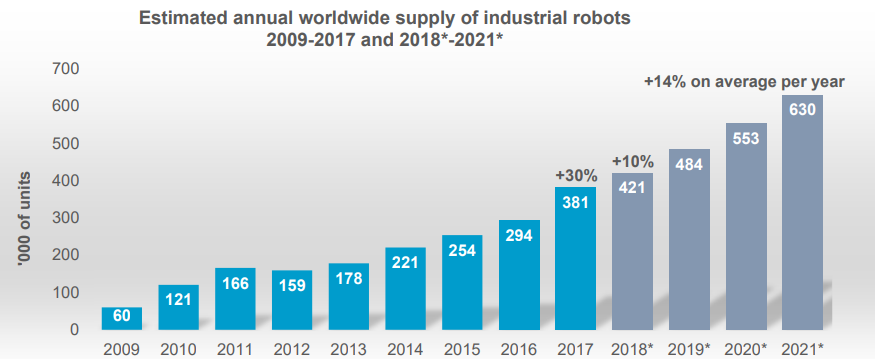
\includegraphics[width=0.8\textwidth]{just_1.png}
	\source{\cite{ifr2018}}		
\end{figure}

\begin{figure}[h!]										\caption{Demanda global de robôs em cada setor da indústria no período 2015-2017} \label{fig:just_2}		
	\centering										
	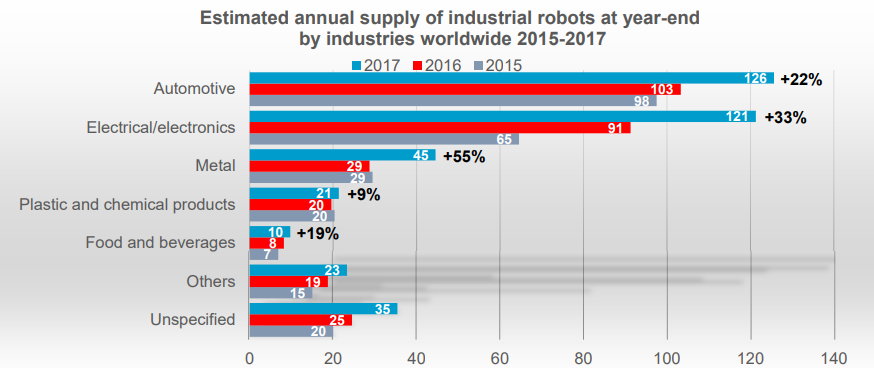
\includegraphics[width=0.8\textwidth]{just_2.png}
	\source{\cite{ifr2018}}		
\end{figure}

Esse aumento na demanda está presente em todas as áreas da indústria, como mostrado na figura ~\ref{fig:just_2}, com maior relevâncias nos setores eletroeletrônico e automotivo, de onde vêm as maiores expectativas de inovação por parte da população.
 
Um exemplo de tecnologia que está sendo desenvolvida nessa área, e que é uma das mais esperadas pelo público, são os carros autônomos, que prometem, além da condução independente, maior segurança para os passageiros e tomadas de decisões importantes como a escolha de rotas e ações para evitar acidentes.

Aliado a isso, existe um aumento na demanda por profissionais qualificados cada vez maior nesse setor. Em adição, há ainda uma notória dificuldade em capacitar trabalhadores para lidar com tecnologias as quais eles não tiveram contato durante o ensino médio e fundamental. Alguns conceitos, que não são novos, como sistemas autônomos, \textit{Machine Learning}, \textit{big data}, tem despertado a curiosidade e estimulando a imaginação da sociedade. Porém, isso vem trazendo alguns equívocos.

Um dos problemas encontrados na formação de profissionais para atuar na área da robótica, é que, diante destes “novos” conceitos as pessoas tendem a se retrair e ter uma noção equivocada, pensando que estes conceitos, que são primordiais para robótica, são extremamente difíceis e complexos, quando na verdade a abordagem de ensino não se preocupa com a desmistificação destes conceitos. É comum ouvir que a automação irá estabelecer novas relações trabalhistas, que irá extinguir alguns empregos e irá criar outros, porém, será que a nossa sociedade está preparada para estes novos empregos? 

Voltando ao campo da pedagogia, foi através de cenários semelhantes à este, que nasceram os movimentos Maker e STEM, oriundos da metodologia Do It Yourself (em português: faça você mesmo). Segundo \cite{Pugliese} ambos valorizam a possibilidade de utilizar das informações obtidas por pesquisa e conteúdo online de fácil acesso para fazer projetos com as próprias mãos. Esses projetos devem fomentar a utilização de equipamentos relacionados à áreas da ciência e da engenharia, seja com ajuda de um computador, impressora 3D ou ferramentas. Essa abordagem visa aumentar a atratividade para as áreas da ciência e desmistificar tabus relacionados à dificuldade de se aprender novas tecnologias.
 
Como resultado, mais jovens e adultos interessam-se por tecnologia, seguem carreiras na área e aumentam o número de profissionais qualificados no mercado.
Ainda no campo da pedagogia, segundo \cite{Mataric} o ensino da robótica é interdependente de aulas no formato da pedagogia clássica, porém melhor aproveitado quando associado a atividades práticas em grupo. Por este motivo considera-se que o movimento Maker e algumas metodologias de ensino de robótica são baseadas na concepção de Lev Vygotsky, onde o sujeito é considerado um ser não só ativo como também interativo, porque adquire conhecimentos a partir de relações intra e interpessoais, exercitando o que o homem tem de melhor: a criatividade.
 
Palangana, \cite{Palangana}, diz que segundo a concepção de Vygotsky, a aquisição de conhecimentos se dá pela interação do sujeito com o meio. Essa associação visa apresentar de forma menos abstrata conceitos abordados nas aulas teóricas e propor compartilhamento de aprendizagem e fomentar o trabalho em grupo entre os alunos dos níveis Fundamental II e Médio.

Analisando a conjuntura atual, uma nova abordagem ao ensino de conceitos básicos de robótica foi idealizada, sendo apresentada como um kit didático de robótica básica aplicada. Este kit terá como principal objetivo o ensino teórico e prático, de conceitos e ferramentas básicas utilizadas no mundo da robótica, em aplicações nos mais diversos setores da sociedade.
 
Tendo em vista o abordado acima, esta monografia tem como objetivo apresentar o projeto de um kit didático de aprendizagem de conceitos básicos em robótica aplicada, utilizando o framework ROS e aplicando conceitos básicos de cinemática e visão computacional.

%--------- NEW SECTION ----------------------
\section{Organização do \thetypework}
\label{section:organizacao}
O documento está organizado em cinco capítulos, seguindo a seguinte estrutura:

\textbf{Capitulo 1 - Introdução}: Faz a contextualização do âmbito no qual a pesquisa proposta
está inserida. Propõe justificar a problemática abordada, e porque a mesma é passível de uma solução. Apresenta, portanto, a problemática, as justificativas e os objetivos deste trabalho.


\textbf{Capítulo 2 - Referencial Teórico}: Apresenta o embasamento teórico que foi utilizado para melhor compor o desenvolvimento do projeto.

\textbf{Capítulo 3 - Metodologia}: Define as etapas de elaboração do trabalho, tal como as metodologias específicas utilizadas em cada etapa do desenvolvimento e suas justificativas.

\textbf{Capítulo 4 - Desenvolvimento}: Apresenta o que foi produzido neste trabalho do ponto de vista de todas as frentes abordadas, partindo das conclusões tiradas para iniciar as confecções dos tutoriais e do kit físico, até o resultado final das mesmas.

\textbf{Capítulo 5 - Conclusão}: Apresenta as conclusões tiradas acerca do que foi desenvolvido e das influências das metodologias utilizadas, tal como possíveis melhorias e expansões futuras.

    \chapter{Fundamentação Teórica}
\label{chap:concep}

\begin{flushright}
	"O orgulho é a fonte de todas as fraquezas,\\ por que é a fonte de todos os vícios." \\
	\ \\
	(Santo Agostinho)
\end{flushright}
\section{Pedagogia}\label{sec:didatica}

Por muito tempo, segundo \cite{saviani}, nas sociedades antigas e medievais, a educação era obtida pela maioria das pessoas através do trabalho, sendo a escola apenas um complemento secundário disponível a grupos seletos da elite. A partir do surgimento da sociedade capitalista e seus processos mercantis que os trabalhadores passaram a precisar de conhecimentos que não se voltavam apenas a técnicas de trabalho manual como cultivo da terra, mas também a relações mercantis e acumulação de capital, ao qual inclui instrumentos de trabalho e, posteriormente, moeda, marcando o início da idade moderna e avanço da ciência.

De acordo com \cite{larchert}, o estudo da didática suma nasceu somente em meados do século XVII, a partir dos estudos pioneiros realizados por Jan Amos Komenský (em latim: Comenius; em português: Comênio), que é considerado pai da didática moderna. Em sua principal obra: Didática Magna, Comenius reuniu os conhecimentos sobre o tema e propôs pela primeira vez um modelo revolucionário de ensino em que os conhecimentos científicos são passados não pela imposição característica da época, mas sim pela satisfação e alegria de ensinar e aprender, segundo \cite{gasparin}. A partir de então, a didática, pedagogia e os modelos de escola passaram a ser ponto de estudo enfatizando a maneira de organizar o ensino e moldada de acordo com as necessidades, exigências e transformações da sociedade ao longo dos anos.

A pedagogia pode ser classificada em quatro diferentes escolas:  Tradicional, Renovada, Tecnicista e Crítica. \cite{larchert} justifica essa classificação de acordo com as características de cada elemento na estrutura didática utilizada, como exposto a seguir.

\subsection{Pedagogia Tradicional}\label{sec:ped_trad}

Do século XVII ao século XIX a didática ficou conhecida como didática tradicional, que se caracteriza por acentuar o ensino humanístico, onde os conteúdos, os procedimentos didáticos e a relação professor-aluno não têm nenhuma relação com o cotidiano do aluno e muito menos com as realidades sociais. Há a predominância da palavra do professor, das regras impostas e do cultivo exclusivamente intelectual \cite{libaneo}.
Segundo \cite{larchert}, sua estrutura organizacional é baseada da seguinte forma:
\begin{quote} - "Homem: compreendido a partir dos ideais de igualdade e liberdade pautados na política liberal.

- Conhecimento: a ciência é a única fonte de conhecimento verdadeiro. O conhecimento enciclopédico é transmitido de uma geração para outra;
	
- Escola: a instituição responsável em preparar os indivíduos para o desempenho dos papéis sociais. Deverá educar para as normas vigentes da sociedade através do desenvolvimento das aptidões individuais, garantindo o preparo intelectual e moral dos alunos;
	
- Método de ensino: instrução organizada na exposição verbal do professor, provocando o acúmulo de conteúdos: 
	
	1º) apresentação da matéria nova de forma clara e completa;
	
	2º) associação entre os conteúdos antigos e os novos;
		
	3º) sistematização e generalização dos conteúdos;
	
	4º) aplicação de exercícios e testes;

- Professor: é o arquiteto da mente, o dono do saber, a autoridade maior responsável pelo ensino, centro do processo educativo;

- Aluno: receptor dos conteúdos transmitidos e do método aplicado;

- Ensino: propedêutico, sustentado nas cátedras, organizado basicamente pela oratória do professor e pela aula expositiva, entendido como a “arte de ensinar” e toda ênfase está na teoria;
	
- Aprendizagem: memorização de conteúdos, acúmulo de saberes transmitidos pelo professor e repetidos nos livros;
	
- Avaliação da aprendizagem: individual, oral ou escrita".	
\end{quote}
Essa pedagogia dominou o Brasil até a década de 1930, mas ainda pode ser visto no cenário atual.

\subsection{Pedagogia Renovada}\label{sec:ped_renov}

A partir da segunda metade do século XX, estudiosos desenvolveram a ideia de que a aprendizagem verdadeira é aquela que nasce dos aspectos sociais, emocionais e cognitivos do aluno, não considerando o ensino como um processo de transmissão, pelo professor aos alunos, de conteúdos prontos, mas uma facilitação da aprendizagem, com o professor na função de estimular o aprendiz a aprender \cite{larchert}. Ela acentua, igualmente, o sentido da cultura como desenvolvimento das aptidões individuais, mas a educação é um processo interno, não externo; ela parte das necessidades e interesses individuais necessários para a adaptação ao meio \cite{libaneo}.

Sua estrutura organizacional é baseada da seguinte forma, segundo \cite{larchert}:
\begin{quote}- "Homem: compreendido a partir da sua existência, indivíduo único no mundo, vive e interage em um mundo dinâmico;

- Conhecimento: produto da existência e da experiência que deverá ser compreendido e socializado;

- Escola: instituição organizadora e articuladora entre as estruturas cognitivas do indivíduo e as estruturas do meio ambiente;

- Método de ensino: aprender experimentando, aprender a aprender;
	
- Professor: facilitador da aprendizagem e do desenvolvimento humano;

- Aluno: o aprendiz é o centro do processo educativo;

- Ensino: orientação individual para o aprender fazendo, através de experimentação, pesquisas, dinâmicas de grupo e oficinas;
	
- Aprendizagem: atividade de descoberta, autoaprendizagem;

- Avaliação da aprendizagem: autoavaliação".
\end{quote}

\subsection{Pedagogia Tecnicista}\label{sec:ped_tecni}

No Brasil, entre 1950 e 1970, ocorre o desenvolvimento industrial e tecnológico, cenário propício para o desenvolvimento do tecnicismo educacional, inspirado nas teorias behavioristas, cujas unidades de análises são respostas e estímulos. O indivíduo, motivado por estímulos planejados com rigor, responderá satisfatoriamente aos comandos propostos. Esta abordagem atende às exigências da sociedade capitalista, industrial e tecnológica, pois, para a sua sobrevivência, a massa de trabalhadores precisa de objetivos rigorosamente planejados, executados e controlados \cite{larchert}.
O autor baseia a estrutura organizacional da seguinte forma:
\begin{quote}- "Homem: produto do meio social;
	
- Conhecimento: resultado da experiência planejada, baseada nos princípios científicos;

- Escola: responsável por qualificar mão de obra para o mercado de trabalho;

- Método de ensino: processo de condicionamento através do estímulo – resposta;

- Professor: especialista de uma determinada área é um técnico capacitado para reproduzir com os alunos as dinâmicas aprendidas;

- Aluno: tem o papel de receber, fixar e repetir as técnicas e seus conteúdos;

- Ensino: diretivo e instrução programada;

- Aprendizagem: fixação do programa aplicado, dos conteúdos decorados e da repetição da técnica;

- Avaliação da aprendizagem: verificação dos resultados dos objetivos propostos".
\end{quote}

\subsection{Pedagogia Crítica}\label{sec:ped_crit}

A partir de meados da década de 70, a sociedade brasileira passou a ter uma visão crítica acentuada quanto ao cenário político autoritário, levando esse pensamento crítico a contestar diversas áreas, incluindo o modelo didático utilizado. De acordo com \cite{martins}, essas discussões deram origem a uma didática que traz como princípio norteador a abordagem crítica da educação, influencia o potencial social dos alunos e professores através de debates, diálogos críticos e considera o ensino nas suas múltiplas dimensões: social, afetivo, cognitivo, motor e político. Estudiosos como Paulo Freire ganharam espaço com proposições de um ensino mais dinâmico e menos alienado, voltado para a libertação do homem. Para \cite{freire}, o diálogo aberto, igualitário e ativo em todos os interlocutores é o principal caminho para a real comunicação, sendo o único capaz de dissipar e gerar conhecimento com eficácia.

De acordo com \cite{larchert}, sua estrutura organizacional é baseada da seguinte forma:
\begin{quote}- "Homem: cidadão e agente de transformação social;
	
- Conhecimento: socialmente referenciado, reflexivo e crítico;

- Escola: construtora de conhecimento crítico que busca a transformação social;

- Método de ensino: dialético, parte da experiência do aluno e do professor, confrontando-a com o saber sistematizado, pautado na dialogicidade, o diálogo como produtor de conhecimento e de emancipação do cidadão;

- Professor: mediador, orientador e agente de mudança social;

- Aluno: aprendiz participativo e crítico;

- Ensino: organização de experiências destacando os conhecimentos da ciência para explicá-las criticamente;

- Aprendizagem: desenvolvimento de estruturas cognitivas e sociais para a emancipação do aluno e do professor;

- Avaliação da aprendizagem: avaliar para mudar; autoavaliação".
\end{quote}
\section{Didática na Sociedade Contemporânea}\label{sec:didatica_sociedade_cont}
A Didática, de acordo com as definições de \cite{libaneo}, é uma das disciplinas da pedagogia, sendo responsável por estudar e investigar, teórica e praticamente, os objetivos, conteúdos, meios e as condições do processo de ensino, a fim de educar o indivíduo no âmbito social. Por ser dependente da sociedade ao qual o indivíduo está inserido, os modelos didáticos estão em constante transformação para adequar a educação ao modelo social vigente em cada época. No entanto, segundo \cite{al-mufti}, os modelos atuais de educação não estão atendendo ao rápido crescimento demográfico e tecnológico do século XXI, sendo necessário uma adequação mundial a uma sociedade globalizada, tecnológica e superpovoada. 

O perfil de aluno contemporâneo é de um indivíduo que cresce em um ambiente sem fronteiras onde parece não haver limites para a velocidade na troca de informações, que ocorre em tempo real, e onde a internet  permite obter qualquer tipo de informação na palma das mãos e de onde estiver. Qualquer questão pode ser respondida com uma simples pergunta no Google, transferindo a fonte de aprendizado e modificando o papel da escola. 

Para atender ao perfil deste aluno é preciso ensiná-lo a buscar o próprio conhecimento através de informações corretas, guiá-lo em meio a infinidade de informação equivocada que ele pode encontrar na web. Parte dessa adequação se passa por abdicar dos modelos didáticos defasados que ainda persistem em dominar as escolas ao longo do globo, incluindo o Brasil, onde existem vestígios do sistema tradicional; e preparar o aluno para se adequar às transformações cada vez mais frequentes do século XXI. Por isso é cada vez mais coerente pensamentos como o de \cite{freire}, no qual diz que estamos numa sociedade em transição precisando romper com o mal da alienação e investir numa educação crítica que adapta e integra o homem ao mundo invés de acomodá-lo e transformá-lo. 

\subsection{Ensino de Novas Tecnologias}\label{sec:ens_novas_tecn}
Na sociedade do século XXI, de acordo com \cite{benitti}, as pessoas estão imersas desde a infância em ambientes com infinidade de informações, de tecnologia avançada e dinâmica que ultrapassam os limites dos laboratórios e englobam as casas, carros, celulares, computadores e todo o entorno, sendo  muito utilizada, mas pouco conhecida pela maioria da população. Este cenário tem expectativa de severidade maior com o desenvolvimento da tecnologia, a chegada da indústria 4.0 e internet das coisas, sendo necessário uma revolução no sistema de ensino para adequar o homem às atividades e profissões do futuro.

Uma forma de viabilizar isso é através da robótica educativa, na qual o aluno é estimulado a desenvolver a sua criatividade, senso crítico, capacidade de elaborar hipóteses, investigar soluções, tirar conclusões e resolver problemas enquanto cria afinidade com conceitos que estão inseridos no seu cotidiano, mas passam despercebidos por boa parte das pessoas. Para tal utiliza-se de softwares didáticos, kits intuitivos e metodologias de ensino baseadas na pedagogia-crítica, onde o aluno é participativo e livre, enquanto o professor é um mediador do conhecimento. Essas metodologias valorizam o trabalho em equipe e desenvolvem a busca própria de aprendizado por mera curiosidade e prazer através de desafios e metodologias DIY (do inglês: Do It Yourself; em português: faça você mesmo) e STEAM (do inglês: science, technology, engineering and Mathematics; em português: ciência, tecnologia, engenharia e matemática), como pode ser visto nos principais kits de ensino de robótica do mercado, por exemplo: Modelix Robotics, Robomind, Mini Maker, Mini Bots e Lego.

\subsection{Movimento STEM}\label{sec:mov_stem}
De acordo com \cite{Pugliese}, STEM education (ou educação STEM, em português) não é exatamente uma metodologia de ensino, mas sim um movimento, resultado de uma transformação maior que muitos sistemas educacionais vêm passando globalmente, decorrente da revolução tecnológica e consequente necessidade de inovação nos modelos de ensino. Este movimento nasceu na década de 1990, quando estudos indicavam que os estados unidos estavam caminhando para um colapso empregatício e econômico somados à escassez de profissionais qualificados nas áreas STEM e um alto nível de desinteresse de jovens alunos nessas áreas. 

Com base nisso, o movimento propõe a reformulação dos métodos de ensino para se adequar à realidade dos alunos, trazendo maior atratividade e incentivando o desenvolvimento de carreiras STEM. Em termos de metodologia, o movimento preza pela aprendizagem baseada em projetos e desafios, estimulando a curiosidade e participação dos alunos. Apesar de ter se difundido com sucesso pelos Estados Unidos e outros países líderes em educação e tecnologia ao redor do globo, o movimento STEM ainda é tímido no Brasil, caminhando a passos curtos com pouco empenho por parte do sistema básico de educação. 

\section{Robótica Educacional}\label{sec:robot_educ}
De  acordo com \cite{nascimento}, a Robótica Educacional, também conhecida como Robótica Pedagógica, é aplicada em ambientes educacionais onde o aluno pode montar e desmontar um robô ou sistema robotizado, proporcionando aos educandos momentos não só de aprendizado, mas de lazer e entretenimento. Esse termo nasceu por volta da década de 1960, através dos estudos de Seymour Papert e sua teoria que defende o uso do computador nas escolas como um recurso atrativo para crianças, e se popularizou entre os jovens a partir da década de 1990 através do movimento STEAM, mas ainda não está bem integrada como uma ferramenta universal de aprendizagem tecnológica em ambientes escolares regulares.
 
Segundo \cite{maisonnette}, a robótica educacional é uma ferramenta interdisciplinar de extremo potencial, que extrapola os limites da sala de aula e instiga o aluno a consultar conteúdo e professores de variadas áreas na busca por uma solução para o seu problema; e é através dessa ferramenta que o aluno constrói o conhecimento através das próprias observações e do próprio esforço, adquirindo uma aprendizagem mais efetiva que se adapta a suas estruturas mentais por ser palpável. Parte dessa otimização na maneira de se aprender está no papel do professor, que deve assumir, segundo \cite{nascimento}, o papel de “problematizador” que ajuda o aluno a buscar de maneira autônoma a solução, bem como estreitar o caminho entre o conhecimento empírico e o conhecimento científico. O mesmo autor diz que, para desenvolver o uso da robótica pedagógica, o aluno deverá identificar um problema e entender como solucionar de maneira ordenada utilizando um robô; em seguida, ele desenvolve a programação e testa; ao fim, o aluno pode observar seus resultados e obter a chance de corrigir seus erros caso não atinja os resultados esperados. 

Aderir ao movimento STEM é o primeiro passo para aplicar a robótica educacional nas escolas, no entanto, existe muito conservadorismo e dúvidas quanto a como aplicar uma metodologia efetiva, levando muitos autores a realizarem estudos na área para comprovar a eficiência de determinados métodos. Analisando alguns desses estudos, foi possível verificar um padrão de boas práticas e uma tendência a escolher determinadas metodologias para ensinar robótica.
\subsection{Project-based learning (PBL)}\label{sec:pbl} 
De acordo com \cite{karahoca}, a PBL (em português: aprendizagem baseada em projetos) é uma metodologia de ensino que aumenta a motivação e promove a auto-orientação enquanto o aluno desenvolve e aplica princípios de pensamento crítico, coleta e analisa dados, investiga e aprimora questões, debate ideias, faz previsões e compartilha suas conclusões e descobertas com os demais; podendo ser construída em oito estágios:
\begin{quote}
1) Envolver os alunos em problemas do mundo real; se possível, os alunos selecionam e definem os problemas. O desenvolvimento de robô seguidor de linha é um dos principais desafios.

2) Requerer que os alunos pesquisem, investiguem, usem habilidades de planejamento, pensamento crítico e resolução de problemas enquanto executam tarefas como: colocar materiais no lugar certo, estabelecer posições de momento e equilíbrio, selecionar materiais elétricos, etc.

3) Requerer que os alunos aprendam e apliquem conhecimentos e habilidades de conteúdos específicos em uma variedade de contextos, enquanto trabalham no projeto aprendendo elementos de circuito, soldando, operando com silício de calor, descascando cabos, etc.

4) Oferecer oportunidades para os alunos aprenderem e praticarem habilidades interpessoais enquanto trabalham em equipes, com adultos em locais de trabalho sempre que possível, havendo seleção de liderança, comunicação e distribuição de tarefas.

5) Dar aos alunos a prática de usar o conjunto de habilidades necessárias para suas vidas e carreiras adultas (como alocar tempo / recursos; responsabilidade individual, habilidades interpessoais, aprendizagem através da experiência, etc.). Propõe-se colocar os alunos sob pressão de tempo e materiais limitados, situação essa que  é comum na vida profissional.

6) Incluir desde o início do projeto expectativas em relação a realizações/resultados de aprendizagem por parte dos alunos e padrões e resultados por parte da escola/estado.

7) Incorporar atividades de reflexão que levam os alunos a pensar criticamente sobre suas experiências e vincular essas experiências a padrões específicos de aprendizagem.

8) Terminar com uma apresentação ou produto que demonstre aprendizado e seja avaliado; os critérios podem ser decididos pelos alunos, por exemplo, corrida de seguidores de linha. \end{quote}

Estas etapas estimulam a criatividade, buscas por conhecimento e aprendizagem através de prazer e satisfação enquanto se diverte buscando resultados.

\subsection{Collaborative Learning ou team based learning (TBL)}\label{sec:tbl} 
A aprendizagem colaborativa ou aprendizagem baseada em times é uma situação em que duas ou mais pessoas aprendem ou tentam aprender algo juntos \cite{dillenbourg}. Através dela os alunos aprendem virtudes de colaboração e união, enquanto compartilham e agregam conhecimentos e trabalham juntos na resolução de problemas em equipe, buscando evolução e resultados coletivos e individuais através de liderança, comunicação, cordialidade e distribuição de tarefas. Observa-se com as conclusões do experimento de \cite{karahoca}, que a aprendizagem colaborativa é importante na robótica educacional, pois equipes que exercem atividades com contribuição coletiva se sobressaem a grupos individualistas nos aspectos de desempenho e aprendizagem individual e coletiva. 

\subsection{DIY - Do It Yourself}\label{sec:diy}
O conceito de DIY (Do-It-Yourself), em português: Faça-você-mesmo, é bem comum na atualidade e se popularizou a partir do início do sec. XXI, através das redes sociais, com o intuito de permitir que qualquer pessoa aprenda a construir, consertar, modificar, fabricar e desenvolver os mais diversos tipos de objetos e projetos de maneira objetiva e sem a necessidade de comprar algo pronto ou de contratar um profissional. Este conceito é muito importante de ser aplicado no ensino de robótica porque permite que qualquer pessoa aprenda a desenvolver um robô sem a necessidade de um ambiente escolar, de um professor ou de conhecimentos avançados na área, podendo aprender na própria casa.

\subsection{Movimento Maker}\label{sec:maker} 
O movimento maker é uma extensão da cultura DIY, sendo originado quando a revista Make Magazine, criada nos Estados Unidos, promoveu a Maker Faire (feira de fazedores). Após o sucesso e repercussão do evento, grandes empresas de tecnologia como Samsung, Intel, Microsoft, Raspberry, Arduino e Microchip começaram a desenvolver tecnologias exclusivamente para atender esse público. Na robótica educacional, o Movimento Maker caminha lado a lado com STEM, pois em ambos, a ideia é inovar, empreender e evoluir. 

De maneira resumida, o movimento Maker valoriza a possibilidade de utilizar das informações obtidas por pesquisa e conteúdos online de fácil acesso para fazer projetos com as próprias mãos, seja com ajuda de um computador, impressora 3D ou ferramentas, visando aumentar a atratividade para as áreas da ciência e desmistificar tabus relacionados à dificuldade de se aprender novas tecnologias. Como resultado, mais jovens e adultos interessam-se por tecnologia, seguem carreiras na área e aumentam o número de profissionais qualificados no mercado.

Ainda no campo da pedagogia, o ensino da robótica é interdependente de aulas no formato da pedagogia clássica, porém melhor aproveitado quando associado a atividades práticas em grupo. Por este motivo considera-se que o movimento Maker e algumas metodologias de ensino de robótica são baseadas na concepção de Lev Vygotsky, a qual diz que o sujeito é considerado um ser não só ativo como também interativo, porque adquire conhecimentos a partir de relações intra e interpessoais, exercitando aquilo que o homem tem de melhor: a criatividade \cite{Palangana} e \cite{rocha}.

Segundo a concepção de Vygotsky, a aquisição de conhecimentos se dá pela interação do sujeito com o meio. Em todos os experimentos, instituições de ensino e produtos voltados a robótica educacional  analisados neste trabalho, dois ou mais dos conceitos acima descritos foram aplicados, demonstrando um padrão de métodos efetivos para ensino de robótica.



\section{Robótica}\label{sec:oque_robo}
\subsection{O que é um Robô}
A partir da primeira Revolução Industrial, houve o advento do uso de máquinas para substituir a mão de obra humana. A busca de cada vez mais automatizar o processo produtivo foi estimulada por diversos princípios, desde os filosóficos, sociais, científicos e  econômicos. Karel Čapek, em 1921, criou a palavra robot a partir da peça RUR (Rossum's Universal Robots), apresentando uma fábrica que criava humanóides (robôs) com o intuito de que sejam obedientes e realizem todo o trabalho físico \cite{wellek}. Na década de 1940, o escritor Isaac Asimov representou o robô com uma imagem um pouco diferente: este foi reapresentado como um dispositivo mecânico com um cérebro programável por humanos, que seguia algumas regras \cite{asimov}. Estas regras são as três fundamentais leis da robótica:

\begin{quote}
1) Um robô não pode fazer mal a um ser humano e nem consentir, permanecendo inoperante, que um ser humano se exponha a situação de perigo;

2) Um robô deve obedecer sempre às ordens de seres humanos, exceto em circunstâncias nas quais estas ordens entrem em conflito com a 1a lei; 

3) Um robô deve proteger a sua própria existência, exceto em circunstâncias que entrem em conflito com a 1a e 2a leis. 
\end{quote}	

\cite{siciliano2010} conceitua que robôs são máquinas que podem substituir humanos em, desde tarefas de esforço físico a, até, tomada de decisões. Atualmente podem ser encontradas máquinas com inteligência artificial que se adequam e tomam decisões a partir de fatores externos, como o ASIMO (Advanced Step in Innovative Mobility) da Honda, que pode ser visto na Figura 01. O primeiro sistema robótico a existir foi o UNIMATE, da UNIMATION Inc.; quando foi instalado na fábrica da General Motors em Nova Jersey na década de 1950, o UNIMATE era utilizado para elevar peças de metais quentes.

\begin{figure}[h!]												
	\centering												
	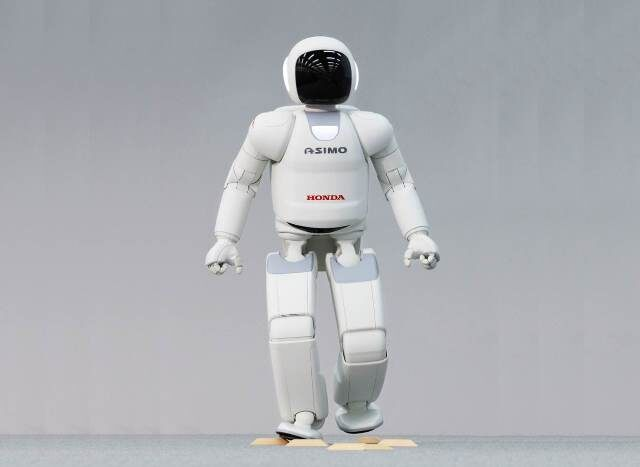
\includegraphics[width=0.8\textwidth]{figura1refbot.png}			
	\caption{ASIMO}		
	\label{img:denavit}	
	\source{HONDA}		
\end{figure}


O uso de robôs industriais como o UNIMATE tem como principal reflexo a automatização da produção, aumentando, portanto, a quantidade de produtos gerados em dado período de tempo. Outro fator que pode ser relacionado ao uso de robôs em linha de produção é a melhora nas condições de trabalho do ser humano, por meio da redução de atividades perigosas ou insalubres \cite{bouteille}.
O controle de sistemas robóticos, com o passar dos anos, vem se tornando mais complexo e especializado, porém pode ser simplificado para um controle de malha fechada, que pode ser visto na Figura 2.2.

\begin{figure}[h!]												
	\centering												
	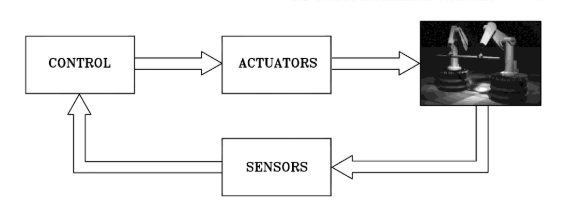
\includegraphics[width=1.0\textwidth]{figura2refbot.png}			
	\caption{Componentes e controle de robôs}		
	\label{img:denavit}	
	\source{\cite{siciliano2010}}		
\end{figure}

Percebe-se, a partir da Figura 2.2 que, em sistemas robóticos, existem atuadores e sensores. Atuadores podem ser citados como sistemas que possuem a capacidade de exercer atuação mecânica para o robô, como o exemplo dos servo-motores. Sensores são transmissores que recebem determinado dado e emitem sinais analógicos ou digitais para o computador central, possibilitando o controle de um sistema robótico. 





\subsection{Percepção}\label{sec:perception}
Segundo \cite{lent}, para a neurociência, a percepção refere-se à capacidade de associar automaticamente as informações sensoriais à memória e à cognição de tal maneira a gerar conceitos sobre o mundo e orientar os comportamentos. Comparativamente, o robô associa os dados “sensoriais” obtidos através dos sensores aos controladores para que possam ser processados e interpretados, dando assim, a capacidade de percepção aos robôs. 

Atualmente, existem diversos sensores que são utilizados, dentre eles: LIDAR, câmeras, IMU, sensores de temperatura, umidade etc. A capacidade de conectar uma ação a partir da percepção de mundo é tarefa do controle, o qual pode emitir comandos de execução para os atuadores a partir das leituras dos sensores. Um exemplo prático disso é o ser humano: quando uma pessoa bate o dedinho do pé, instantaneamente, as terminações nervosas (sensores) emitirão sinais ao cérebro (controle), que por sua vez, emitirá um sinal para os músculos (atuadores) se moverem a fim de interromper a sensação dolorosa.    

A visão computacional é a tentativa de simular a visão biológica, o que se torna em um assunto extremamente complexo. \cite{jahne} escreve que pode-se comparar as funcionalidades básicas dos dois tipo de visão, que são:

\begin{itemize}
	\item Fonte de radiação: sem a emissão de radiação nada pode ser observado ou processado;
	
	\item Câmera: dispositivo que captura a radiação emitida;
	
	\item Sensor: dispositivo que converte a radiação capturada em sinal apropriado para o processamento;
	
    \item Unidade de processamento: dispositivo que processa os sinais convertidos extraindo informações adequadas para a medição do objeto e categorizá-las em classes;
    \item Atuadores: utilização as informações processadas para realizar alguma ação.
    
\end{itemize}

Após esclarecidas as principais funções básicas da visão, também é necessário entender que a visão computacional não é somente o processamento de imagens. O processamento de imagens recebe uma imagem como entrada, e como saída tem-se um conjunto de valores numéricos que podem ou não formar outra imagem. Já a visão computacional é a busca de simular a visão humana, em que a entrada é uma imagem, e a saída é a interpretação dela. 

\cite{gonzalez} escrevem que não existe uma fronteira bem definida entre o processamento de imagens e a visão computacional. Porém é possível dividir o caminho entre o processamento de imagem e a visão computacional em três partes: nível baixo, nível médio e nível alto. O nível baixo é de processos primitivos, como pré-processamento de imagem para redução de ruídos, aprimoramento de contraste e nitidez da imagem. Já o nível médio é caracterizado por processos que têm como entrada imagens, mas a saída do processamento são atributos extraídos da imagem, como arestas, contornos e identificação de objetos. O nível alto trata-se dos processos que interpretam um conjunto de objetos reconhecidos na imagem, desta maneira, realizando funções cognitivas que geralmente são associadas à visão biológica.

\begin{figure}[h!]												
	\centering												
	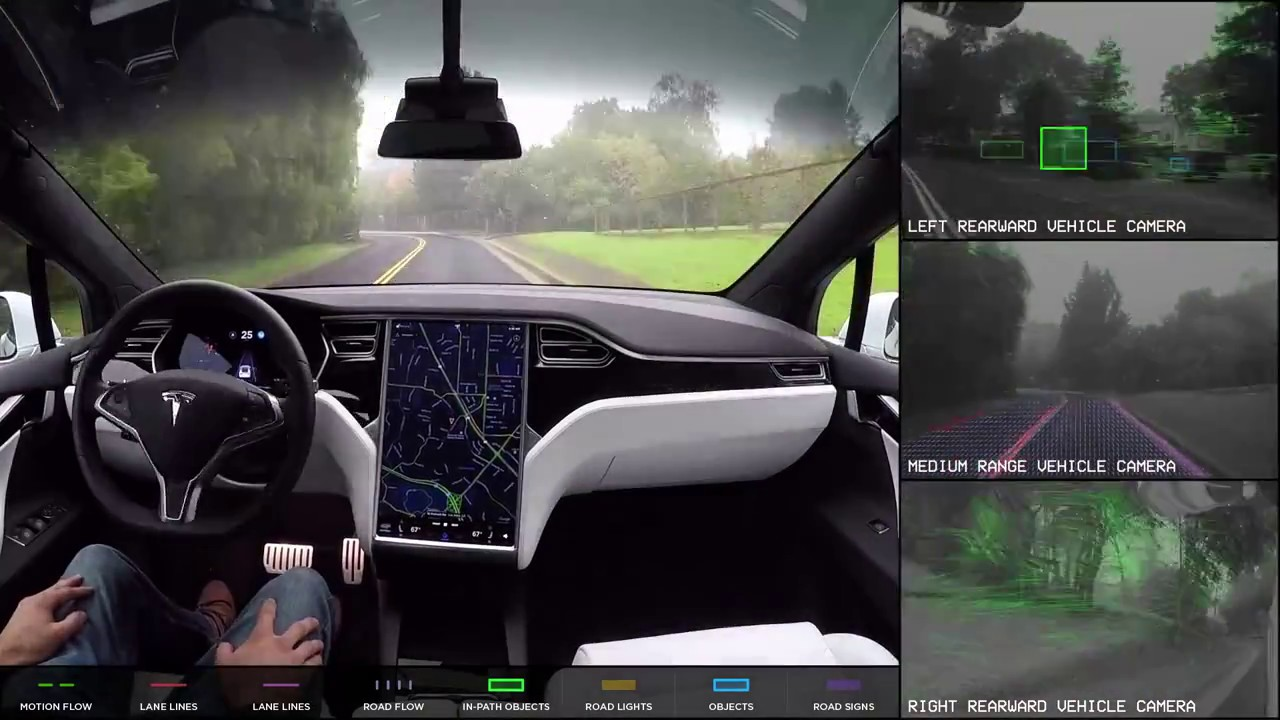
\includegraphics[width=1.0\textwidth]{figura3refbot.png}			
	\caption{Visão da câmera - Piloto automático}		
	\label{img:denavit}	
	\source{Tesla}		
\end{figure}

As aplicações da visão computacional são bastante amplas, e pode ser usada desde para o aumento da produtividade de uma linha de produção através da rápida inspeção, até para que robôs possam compreender seus arredores. Um bom exemplo da utilização da visão computacional é nos veículos autônomos, em câmeras, como podem ser vistos na Figura 2.3, são utilizadas em conjunto com outros tipos de sensores para possibilitar que o automóvel utilize o piloto automático. 



Para que um robô móvel seja autônomo, deve ser capaz de perceber o ambiente à sua volta para que assim possa decidir sobre qual a melhor ação a ser tomada e realizá-la com o menor erro possível. Desta maneira, um das funções fundamentais do robô a fim de alcançar seu objetivo, tanto em ambientes externos quanto em ambientes internos, é a aquisição de informações do ambiente em que está localizado através da construção de mapas do local. Segundo \cite{murphy} os mapas utilizados para navegação dos robôs podem ser classificados, de acordo com sua estrutura, em dois tipos:

\begin{itemize}
	\item Topológicos: modelo que representa o ambiente por meio de conexão entre pontos de referência. A representação pode ser feita por meio de grafos onde os vértices representam os locais e as arestas representam o caminho entre os locais. Porém esse tipo de representação é pobre em detalhes do ambiente físico;
	
	\begin{figure}[h!]												
		\centering												
		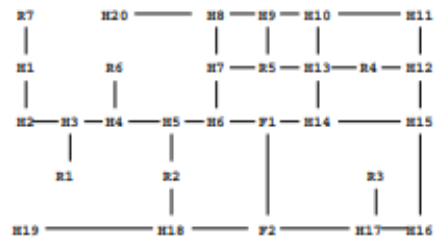
\includegraphics[width=0.6\textwidth]{figura4refbot.PNG}			
		\caption{Mapa topológico de um layout de escritório
		}		
		\label{img:denavit}	
		\source{\cite{murphy}}		
	\end{figure}
	
	\item Métricos: modelo que representa o ambiente físico em detalhes. A representação do ambiente é normalmente feita através de um plano dividido em células de tamanhos iguais, que também é chamada de grade. Desta maneira, cada célula representa uma parte do espaço físico.
	
	\begin{figure}[h!]												
		\centering												
		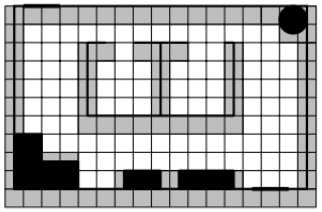
\includegraphics[width=0.7\textwidth]{figura5refbot.PNG}			
		\caption{Grade regular
		}		
		\label{img:denavit}	
		\source{\cite{murphy}}		
	\end{figure}
	
\end{itemize}

\subsection{Controle}\label{sec:control}

Após realizada a percepção do robô, deve-se criar uma estratégia para controlá-lo. Segundo \cite{siegwart} um robô com rodas diferenciais é um robô móvel cujo movimento é baseado em duas rodas motorizadas acionadas separadamente, com cada roda posicionada em ambos os lados do corpo do robô, assim como evidenciado na Figura 06. Esta configuração permite a movimentação em apenas algumas direções, obrigando o robô a fazer uma manobra caso seja necessário alterar a trajetória. O mecanismo que altera esta trajetória é o controle das velocidades das rodas. Por exemplo: caso seja necessário fazer a curva para esquerda, será preciso reduzir a velocidade da roda esquerda, o que é possibilitado pelo acionamento dos motores separadamente. 

	\begin{figure}[h!]												
		\centering												
		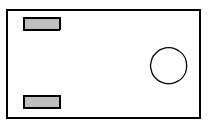
\includegraphics[width=0.6\textwidth]{figura6refbot.png}			
		\caption{Robô com rodas diferenciais
		}		
		\label{img:denavit}	
		\source{\cite{siegwart}}		
	\end{figure}

\subsection{Marcos Fiduciais}
De acordo com \cite{lightbody}, um marco fiducial é qualquer objeto colocado no campo de visão de uma imagem que tem o intuito de ser usado como ponto de referência ou medida.

Atualmente alguns marcos fiduciais mais tecnológicos vem sendo desenvolvidos para funcionarem como apontadores de informações, como por exemplo os QR Codes, que podem ser usados para apontar a um endereço digital específico. Há ainda a capacidade de carregar informações de localização de GPS em marcos fiduciais. Um exemplo dessa aplicação é o uso de ArUco Tags ou April Tags que retornam informações de sua localização relativa a algum outro objeto quando encontrados.

\subsection{ROS}
Segundo a Open Source Robotics Foundation \cite{ros}, o ROS, do inglês \textit{Robotic Operating System}, é um sistema operacional para robôs público, gratuito e colaborativo.

\section{Métodos de projeto}
\subsection{Manufatura aditiva}
A manufatura aditiva é um processo de fabricação tecnológico capaz de criar objetos físicos a partir de um modelo digital. O seu impacto no mundo cresceu exponencialmente na última década, possibilitando a criação de objetos para as áreas da medicina, arte, culinária, indústria e, é claro, a robótica. 

Dentre as tecnologias utilizadas hoje na manufatura aditiva, o grupo optou pela FDM (Modelagem por Fusão e Deposição). Nessa estratégia, um filamento plástico derretido é extrusado sobre uma mesa para formar a primeira camada da peça, e o procedimento se repete camada sobre camada, em alta precisão, até que o objeto seja finalizado.

	\begin{figure}[]												
		\centering												
		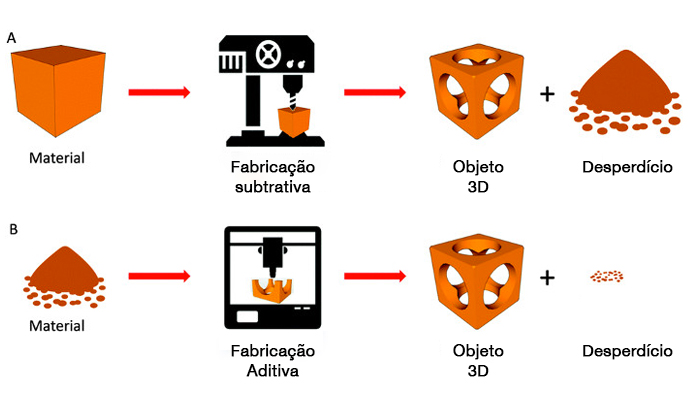
\includegraphics[width=1\textwidth]{impressao.jpg}			
		\caption{Robô com rodas diferenciais
		}		
		\label{img:impressao}	
		\source{\cite{Imp}}	
	\end{figure}
	
	A figura \ref{img:impressao} representa o fator economico diante da impressão 3D, em que este tipo de manufatura se faz mais viável economicamente quando se trata de material. Atualmente, há diversos estudos que visam a utilização da manufatura aditiva com aços, a fim de conseguir estruturas complexas e processes de manufatura mais baratos.
    \chapter{Metodologia}
\label{chap:meto}
\begin{flushright}
	"Tudo o que temos de decidir é o que fazer com o tempo que nos é dado." \\
	\ \\
	(Gandalf)
\end{flushright}
    \chapter{Desenvolvimento}
\label{chap:desen_test}
\begin{flushright}
	"Sou eu, ou o mundo está ficando cada vez mais louco?" \\
	\ \\
	(Coringa)
\end{flushright}

Para obter de forma efetiva o proposto na metodologia, foram elaborados dois conjuntos principais de entregáveis: os Tutoriais, e o Kit Físico. Após finalização do projeto, os Tutoriais se encontram em domínio virtual, na Wiki do repositório da Learnbotics no Github, e o Kit Físico foi fabricado e montado. A seguir encontra-se uma melhor explicação de como esses resultados foram obtidos.

\section{Preparação do Hardware}
Para que tudo o que foi pensado pelo projeto pudesse ser desenvolvido e passado ao usuário, uma escolha cuidadosa do hardware foi efetuada. Posteriormente, uma configuração e testes deste hardware foram também realizados.

\subsection{Componentes de Hardware}

\subsection{Configuração da Raspberry Pi}

\subsection{Componentes de Software}

\subsection{Testes de Hardware e Software}

\section{Tutoriais}
De forma a melhor organizar a elaboração do conteúdo dos tutoriais, uma divisão dos mesmos foi feita de acordo com o assunto abordado, ocasionando assim uma menor abrangência de assuntos a serem pesquisados, de conteúdos a serem concentrados e de novas interpretações a serem elaboradas. As subseções a seguir tratarão de partes específicas dos tutoriais.

\subsection{Um Breve Histórico da Robótica}
siaufgasiogfçwaugfsçfçsuaigfawgfçksgfiauçgwfgsfsaf fsiuafawfioashf saif sfiaywo fasfhaufaw fsifshaf wif saif w

\subsection{Introdução à Robótica atual e Alguns Conceitos Básicos}

\subsection{Introdução à Atuação}
Para que o estudante possa compreender de uma forma mais aprofundada o que está fazendo, antes de começar a mexer com os Dynamixels, uma pequena introdução a atuação foi elaborada.

Essa Introdução trata de uma forma simplificada do conceito de atuadores, de tipos de atuadores, de conversão de energia, e apresenta exemplos cotidianos de atuadores explicando seu funcionamento e aprofundando um pouco mais os conceitos de conversão de energia.

COLOCAR IMAGEM DA WIKI???? 

\subsection{Introdução à Visão Computacional}

\subsection{Tutoriais da Raspberry Pi}

\subsection{Tutoriais dos Dynamixels}
Após ter tido contato com o conceito de atuadores, o estudante irá encontrar também um tutorial que faz uma introdução aos servo-motores inteligentes Dynamixel$^{TM}$.

Neste tutorial são apresentados os servo-motores inteligentes, suas diferenças para servo-motores comuns, suas vantagens sobre os comuns, qual o papel destes servo-motores no robô e no kit físico e mais precisamente porquê escolhemos utilizar os Dynamixels, e não servo-motores comuns.

COLOCAR IMAGEM DA WIKI????


\subsection{Tutoriais do ROS}
Tendo em vista a ídeia de apresentar ao estudante ferramentas que são de fato utilizadas por profissionais da área, buscamos realizar um material completo sobre as partes iniciais de utilização do framework ROS.

Devido ao nível de conteúdo que é abordado nos tutoriais nativos do ROS, foi feita uma análise de relevância dos conteúdos e uma reescrita completa do conteúdo abordado, trazendo novas abordagens para passar esse conhecimento para o estudante.

Este tutorial foi dividido em quatro partes, sendo elas, em ordem:
\begin{itemize}
	\item Introdução: O que é o ROS e como funciona;
	\item Conceitos Básicos: Apresentação de terminologia e conceitos base utilizados pela comunidade do ROS.
	\item Entendendo como Funciona o ROS: Apresentação de conteúdo novo que foi elaborado com base em analogias para facilitar o entendimento do estudante sobre a ferramenta.
	\item Tutoriais do ROS: Os Tutoriais de fato, onde o aluno irá aprender a configurar e utilizar o ROS.
\end{itemize}

A parte quatro, ou parte dos tutoriais de fato, aborda todos os conceitos de nível iniciante apresentados nos tutoriais oficiais do ROS. Porém estes conceitos foram demonstrados de forma mais simplificada, com linguagem mais simples e de forma acompanhada passo a passo para uma melhor assimilação do estudante.

COLOCAR IMAGEM DA WIKI????

\subsection{Apresentação dos Scripts de Cinemática}
Nesta parte dos tutoriais o estudante terá acesso ao programa que fará com que o seu robô ande. Além disso será ensinado também como o estudante deve proceder para que transforme seu código em um código executável e para rodá-lo.

De forma a estimular o estudante, uma análise mais minusciosa do código, com comentários parte a parte também foi feita. A partir da explicação do que os comandos do programa fazem o estudante terá condições de alterá-lo para concluir etapas e descobrir coisas por si só.

Para finalizar, o tutorial apresenta um desafio para que o estudante de fato assimile o que lhe está sendo proposto, alterando o código e vendo na prática o que isso ocasiona.

COLOCAR IMAGEM DA WIKI????


\subsection{Introdução ao OpenCV}

\subsection{Apresentação dos Scripts de Visão Computacional}

\subsection{Integração dos assuntos anteriores}

\subsection{Desafio Final}

\subsection{Tutoriais de Montagem do Robô}

\section{Kit Físico}

\subsection{Design}

\subsection{Fabricação}

\subsection{Montagem}
 




    %\include{Chapters/ChapterFive}
    %\include{Chapters/ChapterSix}
    %\include{Chapters/ChapterSeven}
    %\include{Chapters/ChapterEight}
    \chapter{Conclusão}
\label{chap:conc}
\begin{flushright}
	"Seja forte nos momentos ruins." \\
	\ \\
	(Coringa)
\end{flushright}

Este trabalho apresentou as prerrogativas e decisões envolvidas na proposição de uma nova abordagem para o ensino da robótica nos níveis não graduados, tal como as metodologias utilizadas, as soluções desenvolvidas e os resultados alcançados durante a execução deste projeto.

Pode-se concluir que o projeto foi finalizado com êxito, uma vez que todos os entregáveis envolvidos foram concluídos, todos os assuntos pedidos foram abordados e todas as ferramentas requisitadas foram incluídas nas soluções apresentadas.

O conteúdo teórico foi escrito em linguagem acessível, e disposto em formato de tutoriais e apostilas disponíveis em domínio virtual. O foco destes tutoriais é apresentar conceitos de uma forma simples, direta e utilizando uma linguagem descomplicada. Ademais, todos os tutoriais estarão disponíveis no Github, em formato de wiki, em repositório aberto, escritos em português, de forma a promover a acessibilidade do conteúdo à comunidades lusófonas em geral.

O kit físico foi dividido em módulos complementares de montagem, resultando em um robô com movimentação diferencial. Por se tratar de um robô simples, que foi
pensado para ser fabricado através de manufatura aditiva, apresenta fácil montagem englobando todos os componentes do kit físico e tangenciando conceitos de poka yoke, a fim de propiciar ao usuário um aprendizado mais amigável. Este kit se torna um diferencial quando estimula o aluno a buscar uma maior interação com a robótica ao passo em que exercita a sua criatividade através de objetos físicos que interagem com conceitos abstratos.

Esta modularização será atrelada à progressão do aluno. Na primeira parte ele terá acesso, principalmente ao computador, aprendendo seu funcionamento básico. Na segunda parte terá acesso aos servomotores e aprenderá a conectá-los ao computador e a enviar comandos a partir de scripts. O próximo passo será adicionar a webcam e aprender a utilizar ferramentas de visão computacional. O estudante continuará tendo acesso a módulos complementares passo a passo a medida que vai avançando nos conceitos, até que chegue ao desafio final que irá integrar todos os passos apresentados anteriormente.

Ao combinar metodologias de ensino diferentes, focando principalmente na parte prática do aprendizado e visando dar forma e visualização a conceitos muitas vezes estritamente abstratos, essa nova abordagem de aprendizado apresenta características apelativas à um público mais jovem. Algumas dessas características que podem ser identificadas são a utilização de uma linguagem mais acessível, e um estímulo à criatividade e ao desenvolvimento de habilidades práticas.

Ao aplicar ferramentas que são utilizadas por profissionais da área, como por exemplo um sistema operacional baseado em Linux, o framework ROS e plataforma de versionamento como o Github, o estudante terá desde cedo contato com conceitos e habilidades requisitadas pelas funções desempenhadas por um profissional da área de robótica.
    % include more chapters ...

   %%----------------------------------------------------------------------------
    %% Include thesis appendices
    %%----------------------------------------------------------------------------

    \begin{thesisappendices}
        %\include{Appendices/qfd}
        %\include{Appendices/arquitetura}
        %\include{Appendices/diagele}
        %\include{Appendices/wireframes}
        %\include{Appendices/logbook}
        %\include{Appendices/bom}
    \end{thesisappendices}

    %%----------------------------------------------------------------------------
    %% Configurar as referencias bibliograficas
    %%----------------------------------------------------------------------------


    \addcontentsline{toc}{chapter}{Referências}
    %\bibliographystyle{abnt-alf}


    \bibliography{References/referencias}

    %%----------------------------------------------------------------------------
    %% Finishing
    %%----------------------------------------------------------------------------

    %\include{Others/ultimafolha}
\end{document}
%%%-------------------------------------------------------------------------------
%%% Here we finished with your thesis formating. Good luck with the contents
%%%-------------------------------------------------------------------------------
